\chapter{Praktická realizácia}
V nasledujúcich podkapitolách si bližšie popíšeme proces realizácie. Ten je však rozdelený na viacero častí. V prvom rade bolo potrebné navrhnúť hardvér. V neskorších fázach softvér. Vo fáze vývoju softvéru sme používali agilnú metodiku bližšie metodiku V, ktorej presný popis je v obrázku.

\begin{figure}[h!]
    \centering
    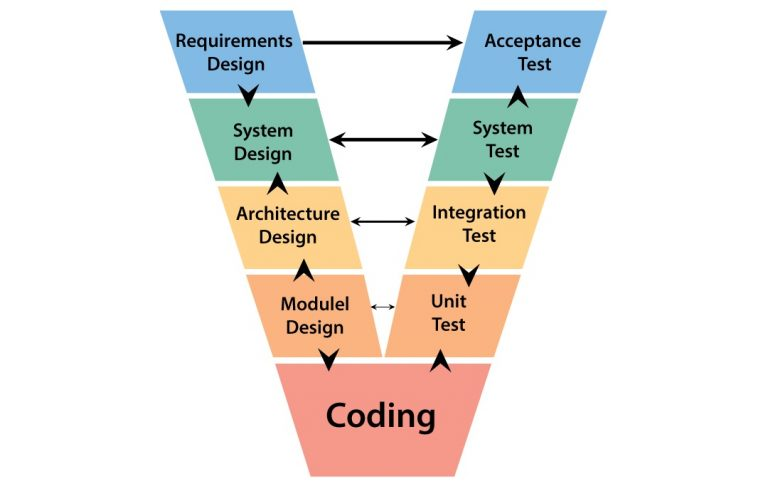
\includegraphics[width=0.6\textwidth]{obrazky/V_model.jpg}
    \caption{V metodika vývoju softvérového produktu}
\end{figure}
Na ľavej strane je vždy vývojový stupeň a na pravej strane je test, ktorý musí prebehnúť k danému vývojovému stupňu. Uprostred je fáza kódovania. 

\section{Hardvérová čast}
% TODO sem vpis podkapitoly kde blizsie popises o tvoreni dosiek
\section{Softvérová čast}
\subsection{Verzovanie súborov}
Všetky programy na ktorých sme pracovali boli uložené vo vzdiaľenom repozitári na serveri GitHub. GitHub je poskytovateľom internetového hostingu na vývoj softvéru a správu verzií s použitím verziovacieho nástroja Git. Ponúka distribuované verziovanie a správu zdrojového kódu systémom Git, ale aj ďalšie vlastné funkcie. Umožňuje regulovať prístup a má niekoľko funkcií zameraných na spoluprácu, ako napríklad sledovanie hlásených chýb, požiadavky na nové funkcie, správa úloh, priebežná integrácia a wiki stránka pre každý projekt.
%https://sk.wikipedia.org/wiki/GitHub
\subsection{Analýza}
Proces analýzy bol celý navrhnutý v programe Enterprise Architect. Kde sme používali \acs{UML} diagramy. Tam sme navrhli celú databázu a vyhľadali sme prípady použitia. Ku ktorým sme zapísali konkrétne scenáre ich aletrnatívy resp. sme použili aj diagramy aktivít. 
\subsection{FrontEnd}
V nasledujucich podkapitolach sa blizsie pozrieme na vyvoj FrontEndu mojej prace. Cely \acs{FE} je implementovany v jazyku \acs{HTML}, \acs{php} a \acs{CSS}. Pre lepsiu pouzivatelsku skusenost sme pouzivali \acl{JS}. Pre vykreslovanie grafov sme pouzili \href{https://grafana.com/}{Grafana}. Pre jednoduchsiu pracu so stylovanim stranky sme pouzili framework \href{https://getbootstrap.com/}{Bootstrap}


\subsection{BackEnd}

\subsection{Databáza}
Na ukladanie zozbieraných hodnôt zo senzorov sme použili databázu. V našom prípade sa jednalo o databázu spoločnosti Oracle s názvom MySQL, ktorá je voľne dostupná a používa ju aj hosting kde je nasadený frontEnd.
\begin{figure}[h!]
    \centering
    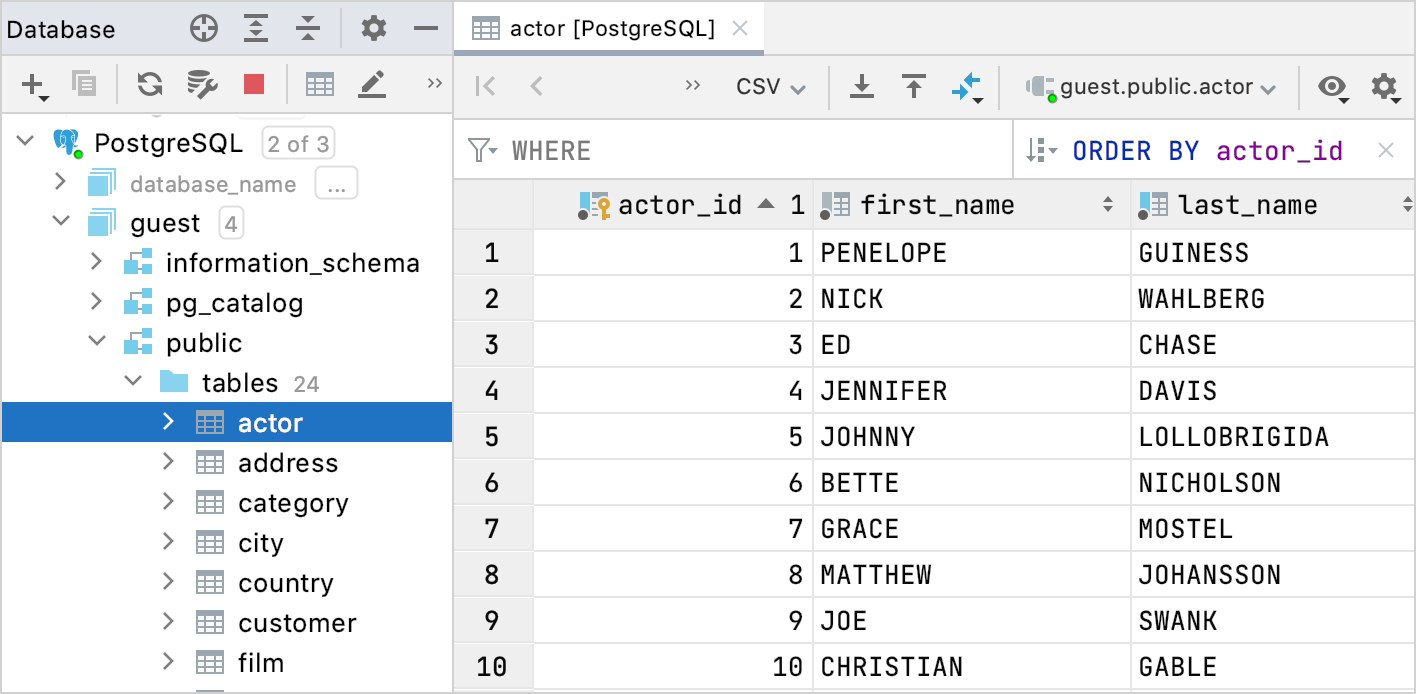
\includegraphics[width=0.6\textwidth]{obrazky/Table.png}
    \caption{Príklad databázovej tabuľky}
\end{figure}

\subsubsection{Návrhová čast databázy}
Pred samotným implementovaním frontEndu je dôležité si určiť podobu databázy. Databázy sa skladajú
\begin{itemize}
    \item tabuľky   
     \item stĺpce
     \item riadky
     \item primárne kľúče
     \item cudzie kľúče
\end{itemize} 
Preto si musíme prejsť celou návrhovou etapou databázy. Tá sa skladá z pomenovania problémových častí. Následne všetky vytypované problémy musíme roztriediť podľa vyššie spomínaného zoznamu.